\chapter{Introduction}\label{chap:Introduction}


This chapter introduces the reader to the concepts of \gls{isomorphic sensing}, \gls{multiplex sensing}, \gls{indirect-imaging}, \gls{task-specific sensing}, \gls{compressive sensing} and \gls{computational sensing}. It also provides the motivation for the need to address the practical issues in experimental computational sensing. 

A \gls{measurement} is a process that converts a physical phenomena to a collection of data. The signal-of-interest is the physical phenomena that we are interested in quantifying. We will call the collection of data the measurement data. Often the measurement is \emph{\gls{isomorphic}}. \Gls{isomorphic sensing} is the concept that a sensor's measurement data resembles the signal-of-interest. \Gls{isomorphic sensing} is called \gls{traditional sensing}. In isomorphic sensing the analog hardware, \acrfull{adc}, and processing algorithms are all seperate components, see Figure \ref{fig:isomorphicsesingflowchart}. \Gls{computational sensing} is the concept that a joint design of the sensor, often though \emph{coding} of the analog signal, with inversion algorithms can exceed the performance of an isomorphic sensor. \Glspl{computational sensor} exist at the intersection of these processes, see Figure \ref{fig:computationalsensingflowchart} \cite{neifeld2006taskSpecificSensing}. While \gls{isomorphic} sensors can provide flexible sensing in multiple applications, a \gls{computational sensor}'s joint design can lead to performance increases. Throughout this chapter and the rest of this dissertation, we will provide many examples that highlight the differences between computational and isomorphic sensing. 

\begin{figure}
    \centering
    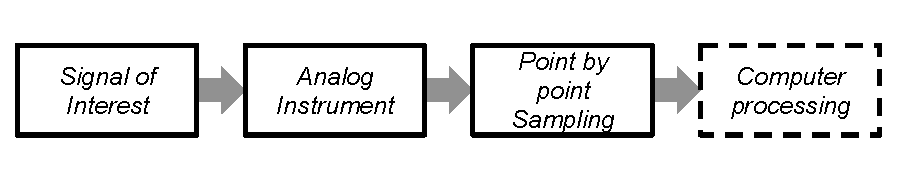
\includegraphics[scale=1]{isomorphicsensorflowchart}
    \caption{A systems view of a traditional sensing scheme. The signal-of-interest is incident upon the analog instrument. The analog instrument forms an isomorphism of the signal which is then periodically sampled point-by-point through an \gls{adc} device. Once the signal is in digital form, post-processing algorithms are often used to perform various tasks such as noise reduction, detection, and classification. Notice that the analog instrument, sampling scheme, and processing are all seperated. }
    \label{fig:isomorphicsesingflowchart}
\end{figure}


\begin{figure}
    \centering
    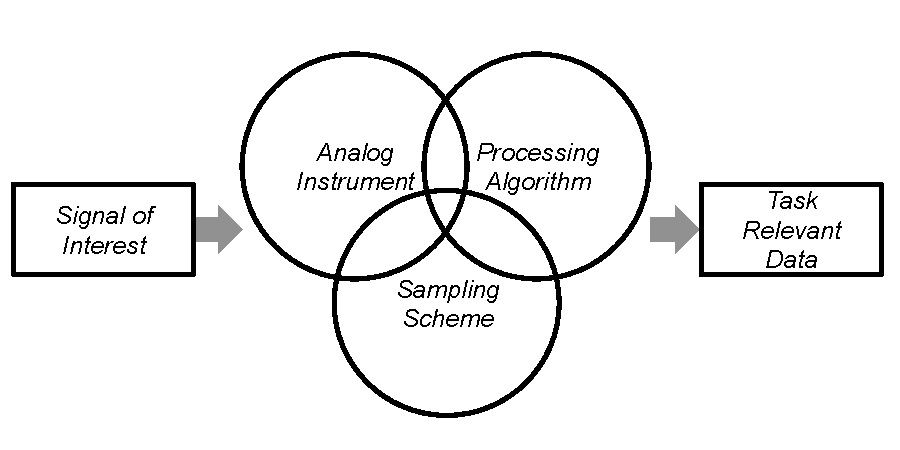
\includegraphics[scale=1]{computationalsensingflowchart}
    \caption{A systems view of a computational sensing scheme. The signal-of-interest is incident upon the analog instrument.  }
    \label{fig:computationalsensingflowchart}
\end{figure}


Rather than a rigorous discussion, this chapter will discuss some of the major developments and concepts in the field of computational sensing on an intuitive level. This will familiarize the reader with important terminology and techniques common in the field of computational sensing. A rigorous discussion with mathematical formalism of the concepts is presented in \autoref{chap:Formalism}. This chapter will also discuss some of the challenges I and many other experimentalists and engineers have faced when developing computational sensing prototypes. I will close this chapter with a brief look ahead to the rest of the dissertation. 

%History%%%%%%%%%%%%%%%%%%%%

\section{Isomorphic Sensing}\label{sec:Isomorphic Sensing}

In Greek, the word isomorphic loosely translates to equal in form. Traditional sensors perform isomorphic sensing. In the context of this dissertation, an isomorphic sensor is any sensor which attempts to produces measurement data that resembles the signal-of-interest. In this paradigm, the analog instrument, sampling scheme, and post-processing algorithms are seperate components and processes.

We will discuss three important examples of isomorphic sensors: the pinhole camera, the photographic camera and the optical spectrometer (which I will just call a spectrometer from now on, even though there are many instruments called spectromers that not concerned with optical spectra). These sensors have had major roles throughout the history of optics and in the physical sciences, so it is natural to use them as examples of computational optical sensing. Therefore it is important we first understand the isomorphic version of these sensors.

In the photographic camera, the signal-of-interest is the object's intensity distribution. This can be the scatter or emitted light from a person, a tree or a distant group of stars. The analog instrument consists of the lenses which are designed and fabricated to produce an intensity disibution (optical image) that looks like the object at the \gls{fpa}. The more that the image resembles the object the better the optics. The \gls{fpa} then samples and quantizes the image and produces a digital representation of the object's intensity distribution, the measurement data. If one is interested in performing a task such as detection or classification, the measurement data is often is post-processed to perform those tasks. 


There are two major sub-systems in the photographic camera which determine how well it performs: the optics and the FPA. Ideally, the optics (the analog instrument in this case) will produce a \gls{psf} which is infinitely small in diameter. For example, in a task such as the detection of a star from several neighboring stars in the night sky, if the \gls{psf} is much larger than the center to center seperation of the two stars in the optical image, it will be quite difficult to detect. A careful reader will note that this is the same argument used by Lord Raleigh in proposing his resolution criterion \cite{rayleigh1879investigations}. Even if the \gls{psf} is small enough, the \gls{fpa} must sample at a fine enough pixel-to-pixel spacing, called the \gls{pixel pitch}, to accurately reproduce the intensity variations at the scale which is pertinant to the task. Intuitively, this makes sense because if the image of the stars are imaged onto a single pixel, then one cannot ever hope to be able to accurately the detect the star without some other prior or side information. 

The pinhole camera consists of a small hole and a box which prevents any light except from the pinhole to enter, see Figure \ref{fig:pinholecamera}. The pinhole camera is useful for imaging in parts of the electromagnetic spectrum and particles for which there is no direct analog to refractive lens or reflective mirror. Like the photographic camera, the pinhole camera also attempts to produce a small \gls{psf} for better spatial resolution and a human observer, film, or \gls{fpa} can be used to measure the object scene. As the hole size decreases, the spatial resolution increase at the cost of reducing the signal strength.

\begin{figure}
    \centering
    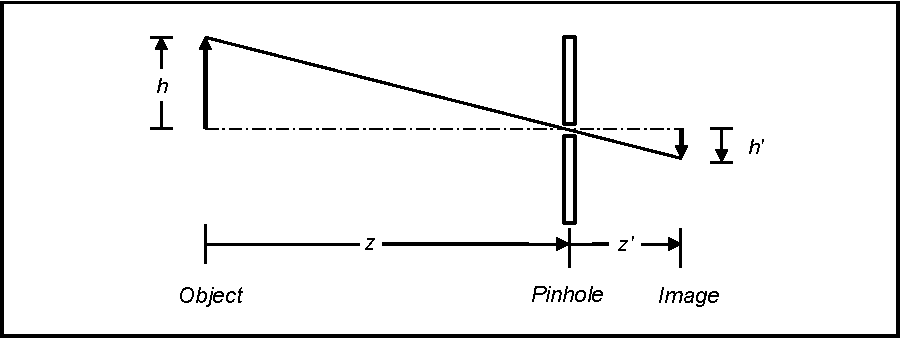
\includegraphics[scale=1]{pinholecamera}
    \caption{A pinhole camera.}
    \label{fig:pinholecamera}
\end{figure}

In the spectrometer, the signal of interest is the spectrum of the object. The optics are designed to take the incoming light and seperate various wavelength components, see Figure \ref{fig:slitspectrometer}. The part of the spectrometer which is used to physically isolate the wavelengths is called a \gls{monochromator}. The result is a spectral intensity as a function of position at the \gls{fpa}. The \gls{fpa} and post-processing algorithms are used in the same manner as the photographic camera, which is to sample the optical spectrum creating a digital version of it and to perform various tasks on the measurement data. For now, we will concentrate on the slit spectrometer, which measures the spectrum at a single point on the object.


\begin{figure}
    \centering
    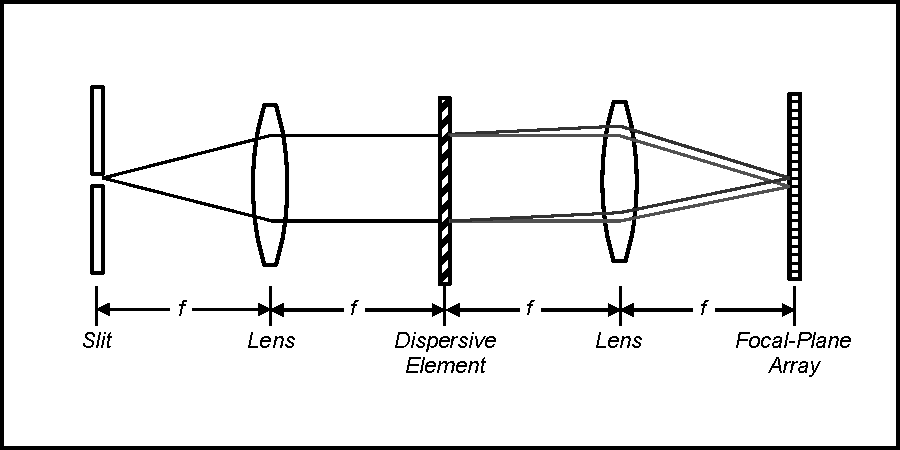
\includegraphics[scale=1]{slitspectrometer}
    \caption{An isomorphic slit spectrometer with a 4F configuration.}
    \label{fig:slitspectrometer}
\end{figure}

In the spectrometer, one of the important performance metrics is \gls{spectral resolution}, which we denote \gls{specres}. The spectral resolution is the smallest difference in wavelength the instrument can discern. Large spectral resolutions can degrade the spectrometers ability to discern important parts of the spectrum. Similarly with the camera, the \gls{fpa} must have a \gls{pixel pitch} which is small enough in order to correctly sample the variations in the spectrum. 

The point-by-point nature of isomorphic sensing is both a strength and a source of weakness. 

The strength comes from the straightforward and intuitive architecture of the isomorphic sensor. Each subsystem: the optics, the \acrfull{fpa}, and the post-processing can be designed and constructed seperately as long as they meet their individual specifications. As long as the \gls{snr} is sufficient and the sampling rate is high enough, we are guaranteed to recover the signal.

One of the weaknessess of the isomorphic approach is the the ability to measure low \gls{snr} signals. Because the signal-of-interest is sampled in a completely parallel fashion at each exposure, each pixel contributes a certain amount of noise. If the noise dominates, the measurement fidelity decreases often forcing the operator to increase the exposure time. For weak signals, the exposure time can become prohibitive and for temporally dynamic signals this may lead to a loss of resolution. Indeed, one of the major engineering trade-offs faced by traditional spectrometer designers is that when one attempts to increase the light collection (increased slit-width) the spectral resolution \gls{specres} degrades. Similarly, in the pinhole camera, there is a throughput versus spatial resolution trade-off, increasing the size of the pinhole degrades the \gls{psf}.

It would be easy to assume that with the recent revolution in machine learning and statistical signal processing combined with the dramatic increase in computing power that we could simply post-process poor measurments and obtain useful data. However, this isn't possible due to the an important theorem in information theory called the \gls{data processing inequality} \cite{cover2012elements}. In layman's terms, it means "garbage in, garbage out".

Another weakness of isomorhic sensing is that the seperation of the analog instrument, the sampling scheme, and the data processing algorithms lead to increased \gls{swap-c}. As we mentioned in the photographic camera, the optics must be designed to produce a small \gls{psf}. For demanding applications, the optical design and fabrication can be the most expensive component of the sensor. While \gls{fpa} prices in the visible have fallen, \glspl{fpa} in certain parts of the electromagnetic spectrum can be quite expensive or non-existant \cite{watts2014terahertz, noor2011compressive}.

In many cases, the signal is redundant and high resolution sampling becomes a waste of resources, such as data storage and communications bandwidth. A good example is in photography where often the post-processing takes the digital image and applies a compression algorithm which looks for patterns in the signal and reduces the file size, discarding much of the sample data \cite{taubman2012jpeg2000}. 

The isomorphic sensor has served humanity well, however with all the weakness that I have discussed, I will now begin to discuss some of major techniques in computational sensing that can be used to address some or all of the issues that I just stated. 

\section{Development of Multiplexing in Sensing}\label{sec:multiplexInSensing}

\Gls{multiplexing} in sensing allows each measurement sample to be a combination of multiple points of the signal-of-interest.  Multiplexing is a powerful tool that can be exploited by the sensor designer to eliminate or relax design trade-offs. 

A simple example which illustrates the usefulness of multiplex sensing is weighing objects. In this example, we are given a 100 sheets of paper. Let's assume that the scale's measurement error is insignificant. Isomorphic measurement sensing means one would need to measure each sheet of paper individually. Requiring 100 measurements. 

Now, let's say the scale's measurement error is on the order of the weight of the sheet. Measuring each sheet invidiually produces a large measurement error. In order to reduce the error to an acceptable \gls{snr} we need to make several measurements per sheet to reduce the error to an acceptable level.

However, we can be a little smarter. We can measure all 100 sheets at the same time. Since the weight of all 100 sheets is much larger than the measurement error of the scale, we can dramatically increase the precision of the measurement. If we can assume that each sheet is the same weight, then we are done. 

The weighing problem is analogous to the spectroscopy example. As discussed earlier in \autoref{sec:Isomorphic Sensing}, there is trade-off between light collection and spectral resolution. Increasing the slit-width to increase the amount of light has the effect of degrading the spectral resolution \gls{specres}. Around the late 1940's and early 1950's, several important papers and inventions demonstrated the effectiveness of multiplexing in spectroscopy. At the time the \gls{fpa} was non-existant, so in the slit spectrometer shown in Figure \ref{fig:slitspectrometer}, where the \gls{fpa} is pictured, there was actually another slit. To record the intensity at each spectral channel, either the dispersive element or the exit slit had to be mechanically translated, making the measurements even slower by a factor of \gls{numspecchan}, the number of spectral channels of interest. 

Golay was the first to propose multiplexing the slit spectrometer by creating a pattern of binary (1's and 0's) entrance and exit slits \cite{golay1949multi}. The idea borrowed heavily from communications theory which is concerned with the reliable transmission of information over a noisey channel. In the Golay multi-slit spectrometer, the patterns of entrance and exit slits are matched based on mathematically useful properties, this is similar to coding and decoding signals in commucations. In communications theory the process of structuring the data from the source to the receiver is referred to as \gls{coding}. Similarly, in computational sensing, the transmission of information between a object signal-of-interest and the sensor is considered a coding problem \cite{brady2009optical}. In the multi-slit spectrometer, the entrance slits act to code the spectrum while the exit slits decoded the coded spectrum. Intuitively, the ability to use multiple entrance and exit slits increases the optical throughput of the spectrometer. Golay's idea dramatically increased the optical throughput without degrading the spectral resolution. 

Another example that is pertinant to this dissertation is coded aperture imaging. Coded aperture imaging can be thought of as the multiplexed version of a pinhole camera. As mentioned earlier in \autoref{sec:Isomorphic Sensing}, there is a trade-off between the throughput and spatial resolution. However in many fields, such as high-energy particle imaging, refractive lenses and reflective mirrors are non-existant or underdeveloped. By using multiple pinholes the throughput is increased without sacraficing spatial resolution. However, the pattern of the pinholes, which is the code, in this case must be carefully designed in order to the reconstruction to be feasible. Fenimore, Canon, and Gottesman were the first to create an elegant solution to coded aperture design called uniformly redundant arrays \cite{fenimore1978coded, gottesman1989new}.

In summary, multiplexing has the ability to eliminate classic trade-offs in isomoprhic sensors: signal strength or resolution. Modern researchers are still actively developing novel ways to implement multiplexing to increase resolution and senstivity in the spatial domain \cite{duarte2008single, townsend2012static}, spectral domain \cite{gehm2006static, tsai2013coded}, and temporal domain \cite{holloway2012flutter,llull2013coded}. However, multiplexing is not without its own set of challenges. As we mentioned, the coding must often be designed to obtain feasible signal reconstruction. We now discuss inverse problems in computational sensing.

\section{Forward Models and Inverse Problems}

In the computational sensing community, a model explains the mapping of the signal-of-interest to the measurement data is called the \gls{forward model}. The problem of taking the observed data and calculating a reconstruction of the signal-of-interst or task-specific parameters is called the \gls{inverse problem}.

As you can imagine, solving inverse problems of isomorphic measurements, when one is concerned with reconstruction of the signal-of-interest, tend to be straight forward. In the weighing problem, the measurement is also the reconstruction. In the slit spectromer, where the forward model can be simply the continuous to discrete mapping of the spectrum. The spectrum is the interpolated measurement. 

Of course, we can begin to add various levels of complexity to the forward model to account for various physical aspects of the sensor, such as the fact the \gls{fpa} can't measure certain wavelength regions or the noise in our measurements. But again, assuming proper sampling and enough \gls{snr}, the reconstruction of the isomorphic signal is the measurement. This simplicity is one reason why isomorphic sensing still dominates at the consumer level despite all of the drawbacks I discussed earlier in \autoref{sec:Isomorphic Sensing}. 

However, the multiplexing of signal information forces us to develop computational steps to solving the inverse problem. In the multiplexed weighing problem, a significant complication occurs when each sheet of paper has a different weight. Now solving the inverse problem is not as straight forward. A single measurement of all 100 sheets in this case is an underdetermined problem, since we have 1 equation and 100 unknowns. What we can do is try measuring different combinations of the 100 sheets, each new combination provides us with a new equation to work with reducing the error. Niavely, we might assume that we can randomly choose 100 unique combinations and solve 100 equations using the algebra we were taught in high school. This works fine when there is no measurement error. However, in the presense of noise, in many applications including the weighing problem, random combinations are not the best way to conduct the coding. They are sub-optimal in terms of reconstruction error. This lead many to begin working on optimal coding strategies of signals for sensing and is major topic in this disseration.

In fact, the idea of multiplexing was not invented by Golay or Fenimore, what they contibuted was the creation of effective ways to code and decode their signal-of-interest, making their sensors more appealling to a broader community of scientists and engineers.

In summary, the forward model of a sensor is essentially accounting for the physics which govern the measurement. While the solving the inverse problem is a mathematical problem which attempts to either reconstruct the object or to calculate task-specific data from the measurement data. Unfortunately, not all multiplexing forward models codes have mathematically elegent inversion steps. Often the physics of the situation force non-isomorphic measurements which require a computational step to solve the inverse problem. 

\section{Indirect Imaging}

While Golay, Fennimore, and others were levering multiplexing to eliminate trade-offs in traditional sensors, an entirely disparate group of researchers were working on imaging techniques for which there was no isomorphic analog. In these cases the physics of the sensing modality prevents a point-by-point sampling of the signal-of-interest. Indirect imaging refer to sensing schemes which include X-ray \gls{ct}, \gls{spect}, \gls{pet}, \gls{mri} and certain forms of sonic and radio wave imaging all require a data-processing or reconstruction step to solve an inverse problem \cite{barrett2013foundations}. 

Perhaps one of the most successful early examples of indirect imaging and the rise of inverse problems in sensing is the development of radar. While early radar was concerned with the detection and distance of an object, development of imaging radar began after World War II. Imaging radar and specifically \gls{sar} can use time delay information combined with the doppler effects and interference patterns of coherent radio waves to create high resolutions of terrain and buildings. 

In medicine, a common imaging modality is X-Ray \gls{ct}. In X-Ray \gls{ct}, computational inversion is required to reconstruct a 2 or 3-dimensional function from 1 or 2-dimensional measurement data. The forward model can be simple: In a collimated beam architecture with a 1-dimensional detector array, we say that each sample from each pixel on the array is proportional to the total number of x-ray photons that have not been absorped by the object \cite{radon20051} plus noise. The inversion of course is not straight forward. The culmination of the work related to the inversion techniques and the actual prototype resulted in the Nobel Prize for Physiology or Medicine in 1979 \cite{nobelprize1979medicine}. 

Indirect imaging is a subfield of computational sensing. Due to the medical or military applications of these computational sensors, there has been an intense push to reduce measurement time and improve task-specific and reconstruction results. Many of the techniques from other subfields of computational sensing have been brought to bear for indirect imaging \cite{zhu2010tomographic, chen2012compressive}. 

We have discussed the development of multiplex sensing and indirect imaging and how the ideas from both subfields are analogous in terms of producing a non-isomorphic measurement. However a major step in practical implementation of computational sensing is being able to obtain the measurements in a quick, reliable and efficient manner. Computational sensing as a field would not exist without the most important invention in optics and photonics of the 20th century. 

\section{The Digital Imaging Revolution}

In 1969 Boyle and Smith invented the \gls{ccd} \cite{boyle1970charge}. The \gls{ccd} is the first integrated circuit device which using a 2-dimensional arrangement of pixels which could reliably convert an intensity distribution to a digital signal. The \gls{ccd} is a type of \gls{fpa}. 

The \gls{ccd} was a major breakthrough for entire fields and industries who depended on the reliable sampling, storage and transmission of optical signals. Until then one either had to use film or bulky tubes that required an electron beam to be scanned across an image scene, such as the Image orthicon \cite{w1975image}. For their invention, Boyle and Smith both received the Nobel Prize in Physics in 2009 \cite{nobelprize2009physics}

The invention of the digital camera by Sasson followed shortly after \cite{kodaksfirstdigital2015}. Several years later the first digital spectrometer was invented. The exit slit was replacing by the \gls{ccd}, whiched allowed for instant and simultaenous measurement of the entire spectrum in a compact architecture \cite{moore1979spectrometer}. 

The development of the \gls{cmos} \gls{fpa} was also important. While in scientific settings, it could not rival the quality of the \gls{ccd}, its cheaper cost brought digital imaging to the consumer level. Other technology like the digital computers and computer networking also provided major contributions to the democratization of imaging and optical sensing. While scientific grade optical instrumentation was and is still expensive, the researcher could at least capture, process, and share measurement data with significantly less effort. Without it, the field of computational sensing would not exist.

Algorithms for efficient and reliable storage and transmission of digital images became more important. Over time the pixel count continued to increase and the sheer volume of digtal image and video data being generated and transmitted over networks began to outpaced improvements in storage and transmission capacity. While many engineers developed new technology to combat the hardware limitations of storage and transmission. This also led to a renewed effort by researchers to develop more efficient image and video compression algorithms \cite{kobayashi1974image, ziv1978compression}. 

While a multitude of compression techniques exist, they all follow the same basic process, see Figure \ref{fig:imagecompressionflowchart}. Once the \gls{ccd} samples the optical signal and produes the measurement data, the encoder usings the compression algorithm to look for redundancies in the data and produce a lower dimensional representation of the image. The compressed data can then either be stored or transmitted or both. The decoder solves the inverse problem of reconstructing the image. 

\begin{figure}
    \centering
    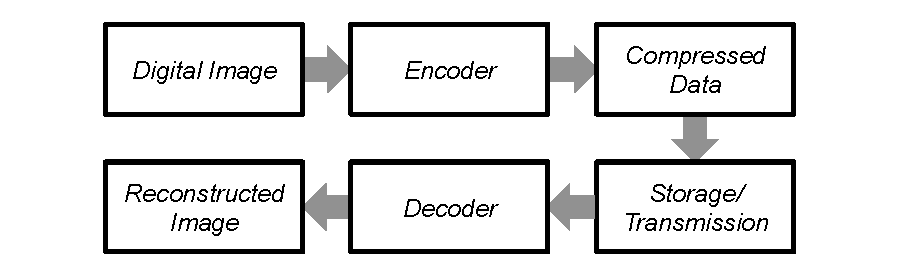
\includegraphics[scale=1]{imagecompressionflowchart}
    \caption{An general flowchart for image and data compression techniques.}
    \label{fig:imagecompressionflowchart}
\end{figure}

As mentioned in at the beginning of this chapter, computational sensing lies at the intersection of the design of the analog hardware, sampling schemes, and processing algorithms. Many of the algorithms used in computational sensing are the same as or inspired by the techniques used by the image processing community. This is because a major effort of computational sensing is the desire to make more resource efficient measurements. 

\section{Compressive Sensing}\label{sec:multiplexingtocompressivesensing}

Traditionally, in order to increase the resolution of a sensor, one had to increase the number of measurements. This means that the \gls{swap-c} must also increase. A camera with just a few megapixels \gls{fpa} costs less than one with hundreds of megapixels. The cost of designing the optics will also need to scale to provide enough optical resolution. In a perfect world, we could capture all the information we need from just a few measurements.

Conventional signal processing dictates that accurate reconstruction of the signal-of-interest is highly improbable. If we have a discrete signal we need at least as many measurements as there are signal elements to solve the inverse problem. If the number of measurements is less, then the inverse problem is underdeterimined. Fortunately, a signal acquisition technique called \gls{compressive sensing} allows us to design sensors that solve these types of highly underdetermined inverse problems.

As discussed earlier, much of the data being generated by sensors are redundant. Images, spectra, video, and audio data of real-world signals tend to exhibit patterns or redundancies that can be exploited. This allows a compression algorithm to significantly reduce the amount of data needed to represent the signal. 

There is a class of compression algorithms called lossy \cite{usevitch2001tutorial}. In lossy compression, not only are redundancies exploited but data that is deemed insignificant to the signal quality is discarded. Only the most important part of the signal is kept as part of the compressed representation of the original signal. When the signal is uncompressed, the amount of data is less that the original measured data. The difference in quality is often unnoticeable to a human observer. In both lossless and lossy compression, the goal is to obtain a \gls{sparse} representation of the signal. A sparse representation means that the signal can be well approximated with only a few non-zero elements in a representation basis. A representation basis is a basis in which the signal-of-interest is sparse. For example, most natural images are sparse in the Fourier basis. The representation basis is typically not the native basis of the signal-of-interest, i.e. pixel number or spectral channel.

In 2006, David Donoho argued that traditional sensors tend to produce vast amounts of measurement data, but often the majority of data is redundant and discarded in the compression step. He proposed that sensors can be designed to directly measure the most relavent data in a signal, suggesting a measurement scheme that can measure a compressed form of the signal \cite{donoho2006compressed}. This is the idea behind \gls{compressive sensing} sometimes known as \gls{compressive sampling}. If the measurements are compressive then it should be possible to significantly reduce the number of measurements to accurately reconstruct the signal. 

Note that there is a subtle but powerful distinction between compressive sensing and the traditional approach of sensing and then compressing. In the traditional approach, compression algorithms operate as a post-processing step. Therefore, a traditional compression algorithm will have access to the entire signal to look for redundancies and convert it into a sparse representation. In compressive sensing, we attempt the compression directly and therefore do not have access to the entire uncompressed signal. The algorithms must assume that the signal has a sparse representation. 

The question of how to actually measure or code the analog signal to directly obtain compressed data is also important. Fortunately, random coding tends to work well in many instances when the signal has a sparse representation. Much of the work in this dissertation will discuss other types of coding schemes that can be used to outperform random codes. 

The idea of compressive sensing seems to be similar to the concept of multiplex sensing. However, there is an important distinction to be made. In compressive sensing, the aim is to obtain the relavent information in as few measurements as possible. In multiplexing, the goal is to overcome limitations mainly due to lack of \gls{snr}. Many compressive sensing schemes also employ multiplexing.

One useful example of compressive sensing versus traditional sensing is the single pixel camera \cite{duarte2008single}. The single pixel camera is a multiplexing camera architecture that uses time sequential random measurements and recovers the image in significantly less measurements (=number of exposures $\times$ pixels) than the conventional camera, see Figure \ref{fig:singlepixelcamera}. Another example is the \gls{cassi} architecture \cite{wagadarikar2008single}, which can reconstruct a spectral data cube in significantly less \gls{fpa} exposures than a traditional spectral imaging architecture. 


\begin{figure}
    \centering
    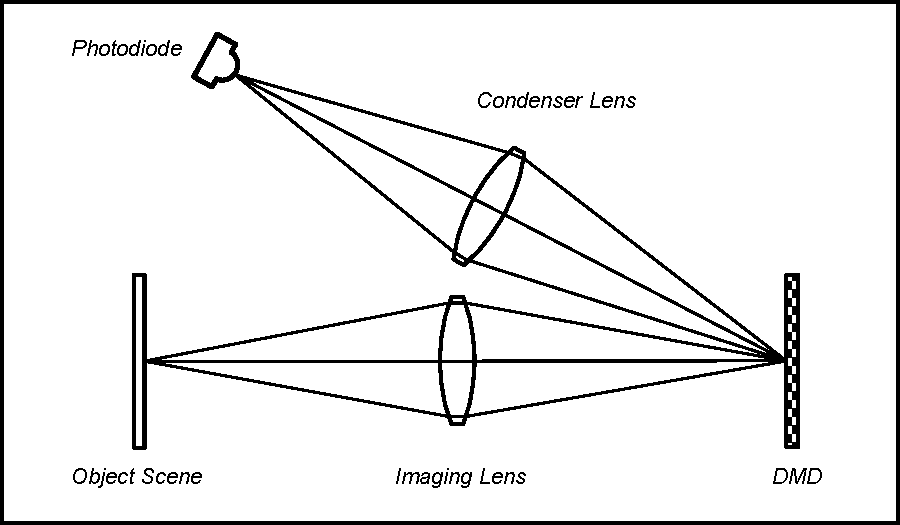
\includegraphics[scale=1]{singlepixelcamera}
    \caption{A single pixel camera architecture.}
    \label{fig:singlepixelcamera}
\end{figure}

Another important distinction is between reconstruction and task-specific sensing. Task-specific sensing tends to refer to measurement techniques that attempt to directly perform tasks such as detection, classification, and estimation without the intermiediate step of reconstructing the high-dimensional signal. Compressive sensing is useful not just of overcoming resolution limitations in reconstruction but for reducing measurement resources for task-specific sensing. For example, in facial recognition the goal is detection of an individual person. Reconstruction of the face image is simply an intermediate step, therefore, one can develop a compressive sensing scheme that is optimal for direct facial detection, skipping the step of image reconstruction \cite{pal2005face}. 

Multiplex sensing, compressive sensing, and task-specific sensing are considered subfields of computational sensing. Computational sensors offer significant advantages that allow us to overcome classic engineering trade-offs in sensor design. However, computational sensing has its own unique set of engineering problems that we will now discuss.

\section{Practical Considerations in Computational Sensing}

So far we have the discussed the development of computational sensing techniques and how they are used to ameliorate trade-offs in traditional sensor design. Computational sensing as a field is continuing to grow at a rapid pace. The number of journal publications related to computational sensings has steadily increases every year since 2008 \cite{stern2016hurdles}. There is now a major OSA meeting dedicated to computational sensing called \gls{cosi} \cite{cosi2016meetingwebsite} and textbooks dedicated to its study and development \cite{brady2009optical, foucart2013mathematical}. It is important to recognize is that while it is a powerful approach to radically new sensor architectures, challenges remain in our ability to design and demonstrate experimental practical computational sensors.

One of the major obstables in computational sensing is calibration. Calibration is the act of quanitying the sensor's measurements in order to produce an accurate forward model. While many traditional sensors also require calibration, computational sensors tend to be more sensitive to calibration error. 

There are two main reasons for this. The first reason is simply due to the fact that non-isomorphic measurements require a computational step to solve an inverse problem. The algorithms rely on accurate knowledge of the forward model to seperate measurement data due to the instrument and data due to the signal-of-interest. 

The second reason is due to the lack of redundancy in a compressive sensor's measurement. The redundancies that are typically deemed wasteful in traditional sensing, can also be used by post-processing algorithms to solve the inverse problem in a robust fashion. If the calibration is wrong for a few measurement sames, one can still use error-correcting algorithms to recover the comprimised data. In a compressive measurement, these redunancies are exploited in the physical measurement process \cite{gehm2013calibration}. Only a few numbers are used to repesent many. If the few numbers are misinterrepted due to poor calibration, the inversion algorithm's performance will suffer. We will illustrate in this dissertation the calibration challenges in several computational sensors. 

Since, calibration has become a major drawback in \gls{compressive sensors}. A consumer cannot be expected to spend time calibrating everytime the instrument is physically bumped or the air pressure changes. In high dimensional compressive sensors like hyperspectral imagers, the calibration time can last hours.

Another hurdle in the implementation of practical computational sensing is the need for prior knowledge. For example, in compressive imaging we have to assume the signal is sparse in some basis. Fortunately most realistic objects are sprase or compressible with modern representation bases, such as the wavelet basis. However, sometimes one needs to image something that is difficult to represent with any current basis, such as the intensity pattern due to laser speckle. One needs an alternative representation basis, so training sets are often used to generate a new basis in which the signal can be represented as sparse. One must generate many different example training data so a particular signal-of-interest can be have a sparse representation in that basis. This becomes time and compuationally expensive. Many algorithms require some prior knowledge of the statistics of the signal and noise ahead of time for optimal performance. A good example of this is the \gls{afssi-c}, a computational spectral classifier which requires knowledge of standard deviation of the noise's probability density function to perform spectral classification in the least number of measurements as possible.

Reducing the number of detector elements is often the goal in computational sensing. A notable example is the single pixel camera is an architecture. However, the single pixel camera requires several time sequential measurements. Each measurement displays a different \gls{dmd} pattern to create a randomly encoded measurements \cite{duarte2008single}. The drawback to this architecture is that one must point the camera at the object scene until enough measurements have been collected for proper reconstruction. A complication arises when this architecture is used to image temporally varying object scenes. One must display the \gls{dmd} patterns even faster and reduce the exposure time to keep up. As a result the \gls{snr} may begin to degrade. 

A possible way to mitigate this issue is to do all the encoding in parallel. However, a completely parallel approach would require a lens, a \gls{dmd} (or coded aperture), and a detector pixel for each measurement. Since each lens uses a different entrance pupil, this will means that each will have a slightly different view of the object scene. This drastically scales the complexity of the architecture and algorithms. In this dissertation, I will discuss a compromise to parallel coding, in two different computational sensors, by using a common entrance pupil and a \gls{ccd}.

Much of the Often, theorectically optimal measurements take advantage of codes which are simultaneously positive and negative. In reality, with incoherent light we are unable to make negative measurements. One is often forced into situations where one must record two sets of measurements and subtract one set of measurements from the positive set of measurements. This means an additional noise term is added to each effective measurement. 

Algorithms engineered to solve the inverse problems often do not account for the non-negativity of many physical situations. For example, in spectral unmixing where the problem is to solve for concentration of each material's spectrum. A non-negative fractional abundance that sums to one is a physical requirement. However, there is a serious lack of sparsity promitting algorithms that are able to enforce both the non-negativity and the sum to one constraint. 

A major issue in both the theoretical and experimental compressive sensing community is a lack of code design schemes. For the most part random measurements techniques are dominant because they obey a key theorectical result which guarantees reconstruction with high probability. Intuitively, designed, meaning non-random, measurement codes which can take into account prior knowledge of the physical limitations of the sensing task and statistical assumptions of the signal-of-interest should be able to outperform random measurements. For example, we will show that in certain applications we can use \gls{pca} to outperform random measurements. In one application, we will demonstrate that simply designed codes outperform random codes in low \gls{snr} environments. However, as of yet there is no adaptive measurement package one can simply take  ``out-of-the-box'' and begin applying them to compuational sensing problems and outperform random measurements on a consistent basis.

These issues and others will be discussed in a case study manner throughout this dissertation. I will now discuss the organization of this dissertation and the three seperate computational sensors I have built and how I have tried to migitate and resolve some of the practical issues associated with computational sensing.

\section{Dissertation Overview}

I used this chapter to cover the major concepts of computational sensing. More importantly, I provided the major topic of discussion for this dissertation, the challenges that are remain towards developing practical computational sensors. I will use the next chapter as an opportunity to provide a more detailed and mathematically rigorous look at the various coding schemes that are popular in computational sensing, as well as the ones I have used. This includes a discussion of the mathematical methods that I and my collaborators developed and deployed in the \gls{afssi-c}: Bayes rule, Log-Likelihood Ratios, and the Maximum a Posteriori decision technique. A more rigourous treatment of compressive sensing will also be provided which includes several important results from the compressive sensing community. I will also talk about several optimization algorithms and estimation techniques that have been used during the development of the three computational sensors in my work.

\Cref{chap:Scout} will introduce a new system architecture for compressive target tracking---the Static Computational Optical Undersampled Tracker (SCOUT). This system is designed to overcome a variety of challenges that typically arise in traditional optical sensing approaches. It provides several advantages over the single-pixel camera architecture, notably it can capture many simultaneous encodings of the field-of-view with a single camera exposure. I will present experimental results that validate the performance of the proposed architecture. 

\Cref{chap:Afssic} will discuss an important experimental protoype which demonstrates adaptive spectral image classification. The system is a major experimental advancement compared to current computational spectral imaging architectures which focus on reconstruction. Furthermore, the ability to perform adaptive measurements, where each code is designed based on the history of prior measurement data allows this instrument to outperform traditional spectral imaging architectures by a factor of 100 in low \gls{snr} scenarios.

\Cref{chap:Csu} will discuss current efforts to experimentally demonstrate compressive spectral unmixing. Often in spectral imaging, the spectra present in the field-of-view of each pixel is actual a mixture of several spectra, a mixed spectrum. Spectral unmixing is the task of inferring the fraction of each constituent spectrum in the mixed spectrum. I employ a unique architecture for computational spectral sensing which uses no diffraction grating or refracting prism but relies on the wavelength dependent nature of the birefringence in an \gls{lcos}. We will demonstrate the effectiveness of various compressive sensing measurement schemes to outperform a traditional sensor in significantly less measurements. 

\Cref{chap:Conclusion} will summarize the dissertation and provide my perspective on how the field should the approach the issues in practical computational optical sensing.


%\bibliographystyle{IEEEtranS}  
%\bibliography{ThesisBib}

